\documentclass[11pt]{article}
\usepackage[margin=1in]{geometry}
\usepackage{graphicx}
\usepackage{enumitem}
\usepackage{parskip}

\title{Engineer Onboarding}
\author{}
\date{}

\begin{document}

\maketitle

\section*{Current Status}
Verified on March 16, 2026 against the live Supabase-backed portal.

Smoke-tested engineer workflows:
\begin{itemize}
  \item login and route protection
  \item engineer dashboard and system status surfaces
  \item settings access
  \item break-glass grant creation
  \item break-glass revoke
  \item redacted family view without active sensitive access
\end{itemize}

\section*{What Engineer Is For}
Engineer is the platform-operations role. This role owns:
\begin{itemize}
  \item system visibility
  \item admin governance
  \item incident tooling
  \item sensitive-access controls
  \item integration and release observability
\end{itemize}

Engineer is not a default ``see everything'' role. Billing and personal data stay redacted until a break-glass grant is opened for a specific support reason.

\section*{Core Boundaries}
Engineer can:
\begin{itemize}
  \item access every main section in the portal
  \item manage \texttt{admin}, \texttt{staff}, \texttt{ta}, and \texttt{instructor} accounts
  \item use role preview
  \item revoke sessions
  \item review system health, drift, and integration status
  \item open and revoke break-glass access
  \item work incident, maintenance, and remediation tooling
  \item manage maintenance banners, change freeze, support notes, and feature flags
  \item inspect read-only schema and system state
\end{itemize}

Engineer cannot do by default:
\begin{itemize}
  \item view billing or family-sensitive detail without break-glass
  \item export sensitive data during break-glass
  \item manage engineer accounts in-app
\end{itemize}

\section*{Screens}
\subsection*{Engineer Dashboard}
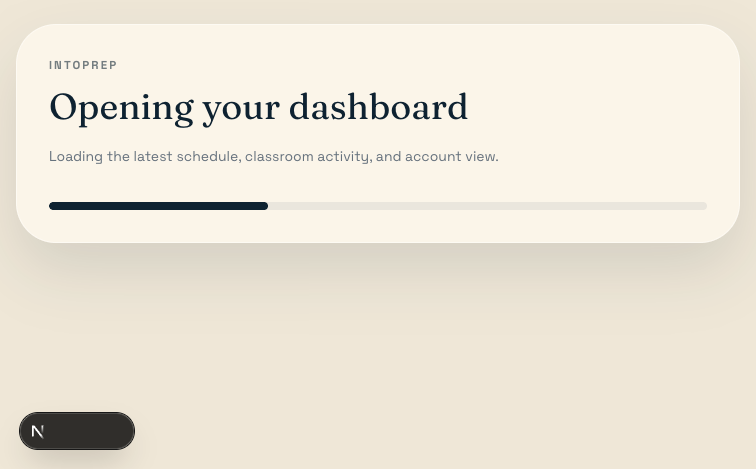
\includegraphics[width=\textwidth]{assets/engineer-dashboard.png}

\subsection*{Engineer Settings}

\includegraphics[width=\textwidth]{assets/engineer-settings.png}

\subsection*{Engineer Family View With Redaction}
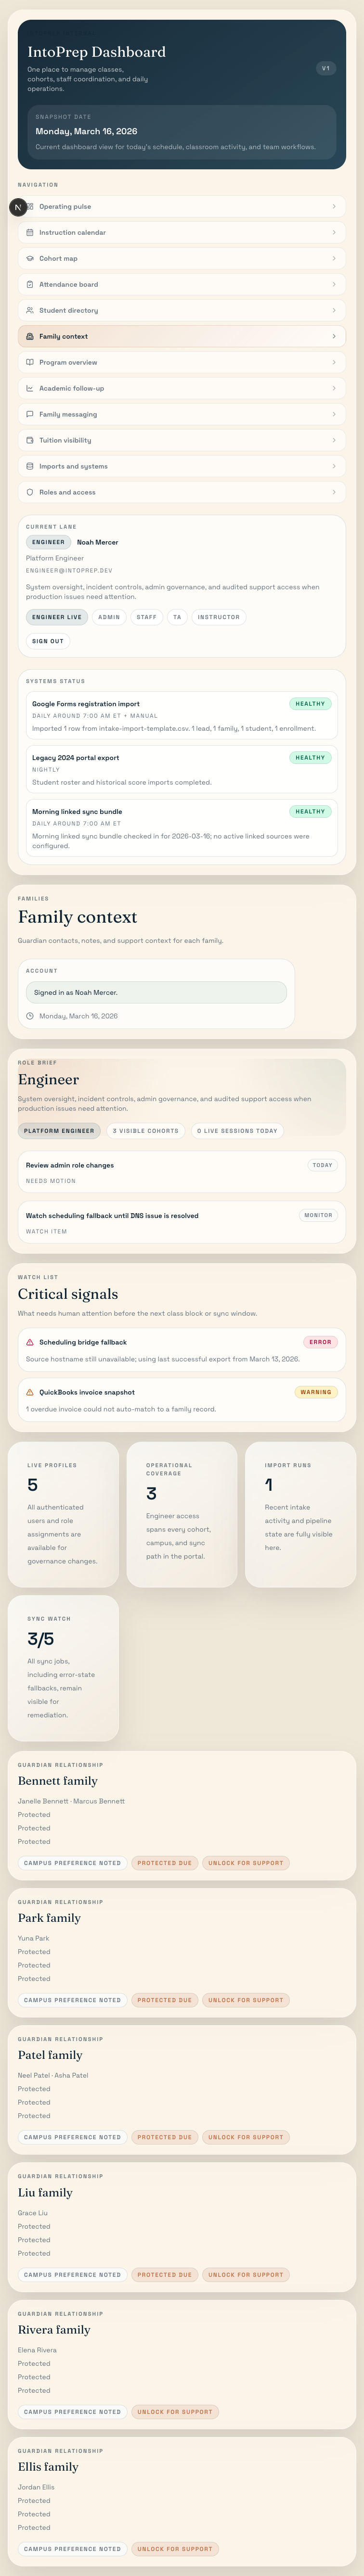
\includegraphics[width=\textwidth]{assets/engineer-families-redacted.png}

\section*{First Login Walkthrough}
\begin{enumerate}
  \item Sign in at \texttt{/login}.
  \item Confirm the left rail shows the full portal navigation.
  \item Start on ``Operating pulse'' and review:
  \begin{itemize}
    \item app version
    \item Git commit
    \item schema version
    \item drift warnings
    \item integration health
  \end{itemize}
  \item Open ``Roles and access'' and verify:
  \begin{itemize}
    \item the managed user list loads
    \item admin accounts are visible
    \item engineer-only controls are present
  \end{itemize}
  \item Open ``Family context'' and confirm sensitive data is redacted until you intentionally open break-glass.
\end{enumerate}

\section*{Daily Workflow}
\subsection*{1. Check System Status}
Use ``Operating pulse'' first.

Review:
\begin{itemize}
  \item release version
  \item schema version
  \item cron health
  \item Google Forms source health
  \item QuickBooks source health
  \item email alert health
  \item recent sync warnings or failures
\end{itemize}

\subsection*{2. Review Governance}
Open ``Roles and access'' and use this screen to:
\begin{itemize}
  \item review active accounts
  \item provision or manage non-engineer roles
  \item manage admin accounts
  \item revoke sessions for compromised non-engineer accounts
  \item review audit activity
\end{itemize}

\subsection*{3. Use Break-Glass Only When Needed}
Open a protected student, family, or billing context only when actively fixing a live issue.

Required inputs:
\begin{itemize}
  \item a clear support reason
  \item the incident or support reference
\end{itemize}

Expected behavior:
\begin{itemize}
  \item the grant is scoped
  \item a timer/banner appears
  \item the grant expires automatically
  \item the grant appears in the active break-glass monitor
\end{itemize}

\subsection*{4. Revoke Access When Done}
From the active break-glass monitor, revoke the grant as soon as the support task is complete.

\section*{Complete Capability Map}
Engineer is the only role that should see the full platform-control layer.

Use engineer for:
\begin{itemize}
  \item platform health and release visibility
  \item schema and config drift review
  \item sync, import, and credential health review
  \item admin governance
  \item session revocation for compromised accounts
  \item break-glass access for sensitive family, student, or billing records
  \item incident acknowledgement, assignment, and maintenance-state actions
  \item remediation actions such as replay, retry, and repair
  \item maintenance banners and feature flags
  \item engineer-only support notes and schema inspection
\end{itemize}

Do not use engineer for:
\begin{itemize}
  \item routine billing follow-up
  \item normal family communication
  \item day-to-day classroom work
  \item local production-data troubleshooting outside the hosted app
\end{itemize}

\section*{How To Use Break-Glass}
\begin{enumerate}
  \item Navigate to the protected family, student, or billing surface.
  \item Select the break-glass action.
  \item Enter:
  \begin{itemize}
    \item a clear support reason
    \item the incident or support reference
  \end{itemize}
  \item Confirm the grant opens.
  \item Verify the banner/timer appears.
  \item Complete the support task.
  \item Revoke the grant from the monitor or let it expire.
\end{enumerate}

\section*{How To Manage Admin Access}
\begin{enumerate}
  \item Open ``Roles and access''.
  \item Search for the target account.
  \item Review current role, status, and recent audit context.
  \item For destructive actions, read the confirmation text carefully.
  \item Complete typed confirmation when prompted.
  \item Confirm the audit log entry appears afterward.
\end{enumerate}

Important:
\begin{itemize}
  \item never remove the last active admin
  \item never use engineer actions casually for day-to-day school operations
\end{itemize}

\section*{How To Revoke A Session}
\begin{enumerate}
  \item Open ``Roles and access''.
  \item Find the affected user.
  \item Confirm the user is not an engineer.
  \item Choose the revoke-session action.
  \item Confirm the action when prompted.
  \item Check the audit log so there is a record of who forced the sign-out and why.
\end{enumerate}

\section*{How To Use Role Preview}
\begin{enumerate}
  \item Start from the left rail role switcher or the preview links in the engineer lane.
  \item Enter the target role preview such as admin, staff, TA, or instructor.
  \item Watch for the preview banner.
  \item Review the visible sections and workflow surfaces.
  \item Exit preview before making live governance or support changes.
\end{enumerate}

Preview is read-only and should be used to validate permissions and user experience, not to operate the business.

\section*{How To Work Incidents And Integrations}
\begin{enumerate}
  \item Start on ``Operating pulse'' and review warning and error states.
  \item Open the relevant sync or integration surface.
  \item Confirm source health, recent run history, and ownership.
  \item If needed:
  \begin{itemize}
    \item acknowledge the issue
    \item assign the issue
    \item add handoff context
    \item retry or replay a failed step
    \item pause a source or move it to maintenance mode
  \end{itemize}
  \item Add a support note if the incident needs shared context for later.
\end{enumerate}

\section*{How To Use Maintenance Banner And Change Freeze}
\begin{enumerate}
  \item Use the maintenance banner when staff should see an internal portal-wide notice.
  \item Keep banner wording plain, operational, and time-bound.
  \item Use change freeze only when risky writes should be blocked during an incident.
  \item Enter a clear reason and issue reference for any freeze.
  \item Remove the banner or freeze as soon as the incident window closes.
\end{enumerate}

\section*{How To Use Feature Flags, Support Notes, And Schema Inspector}
\begin{itemize}
  \item Feature flags:
  use them to roll out internal behavior changes by role without affecting everyone at once.
  \item Support notes:
  use them for engineer-only troubleshooting context tied to incidents, accounts, or integrations.
  \item Schema inspector:
  use it for read-only data and schema verification when the UI and database state appear out of sync.
\end{itemize}

These tools are for platform operations only and should not replace normal admin or staff workflow.

\section*{What To Watch During Incidents}
\begin{itemize}
  \item drift between app version and schema version
  \item incomplete integration setup
  \item failed or warning-state syncs
  \item repeated billing or intake mismatches
  \item unusual session or account activity in the audit log
\end{itemize}

\section*{Guardrails}
\begin{itemize}
  \item sensitive access is audited
  \item dangerous actions require explicit confirmation
  \item engineer activity should stay inside the hosted app for production investigations
  \item local development should stay on synthetic or isolated local data
\end{itemize}

\section*{Verified Behavior}
Verified in the live browser pass:
\begin{itemize}
  \item engineer login succeeded
  \item engineer could access ``Roles and access''
  \item engineer could create a scoped break-glass grant
  \item engineer could revoke that same grant successfully
  \item sensitive family context stayed redacted before grant access
\end{itemize}

\section*{Not In Scope For Normal Engineer Use}
\begin{itemize}
  \item direct family operations
  \item routine billing follow-up
  \item staff task execution
  \item TA classroom support work
  \item instructor teaching workflows
\end{itemize}

\section*{Recommended First-Day Checklist}
\begin{itemize}
  \item review ``Operating pulse''
  \item open ``Roles and access''
  \item inspect the audit log
  \item test one break-glass grant and revoke flow on a real support case when needed
  \item review current drift and sync warnings before governance changes
\end{itemize}

\end{document}
\ No newline at end of file
